\providecommand{\main}{../../..}
\providecommand{\Figures}{\main/Figures}

\documentclass[\main/main.tex]{subfiles}

\begin{document}
            
\section{pz{}, le second modèle le plus utilisé en laboratoire}

%%
%
Le \pz{} est une espèce de poisson d'eau douce originaire d'Asie et très commune au nord de l'Inde.
%
Il appartient à la famille de Cyprinidae, comme la carpe commune.
%
Il s'agit du second organisme modèle le plus employé.
%
Presque quatre milles publications ont utilisé le mot "zebrafish" en 2019
selon PubMed(voir Figure~\ref{fig:model:pz:stats}).

\begin{figure}[htbp]{\textwidth} 
    \centering
       \centering 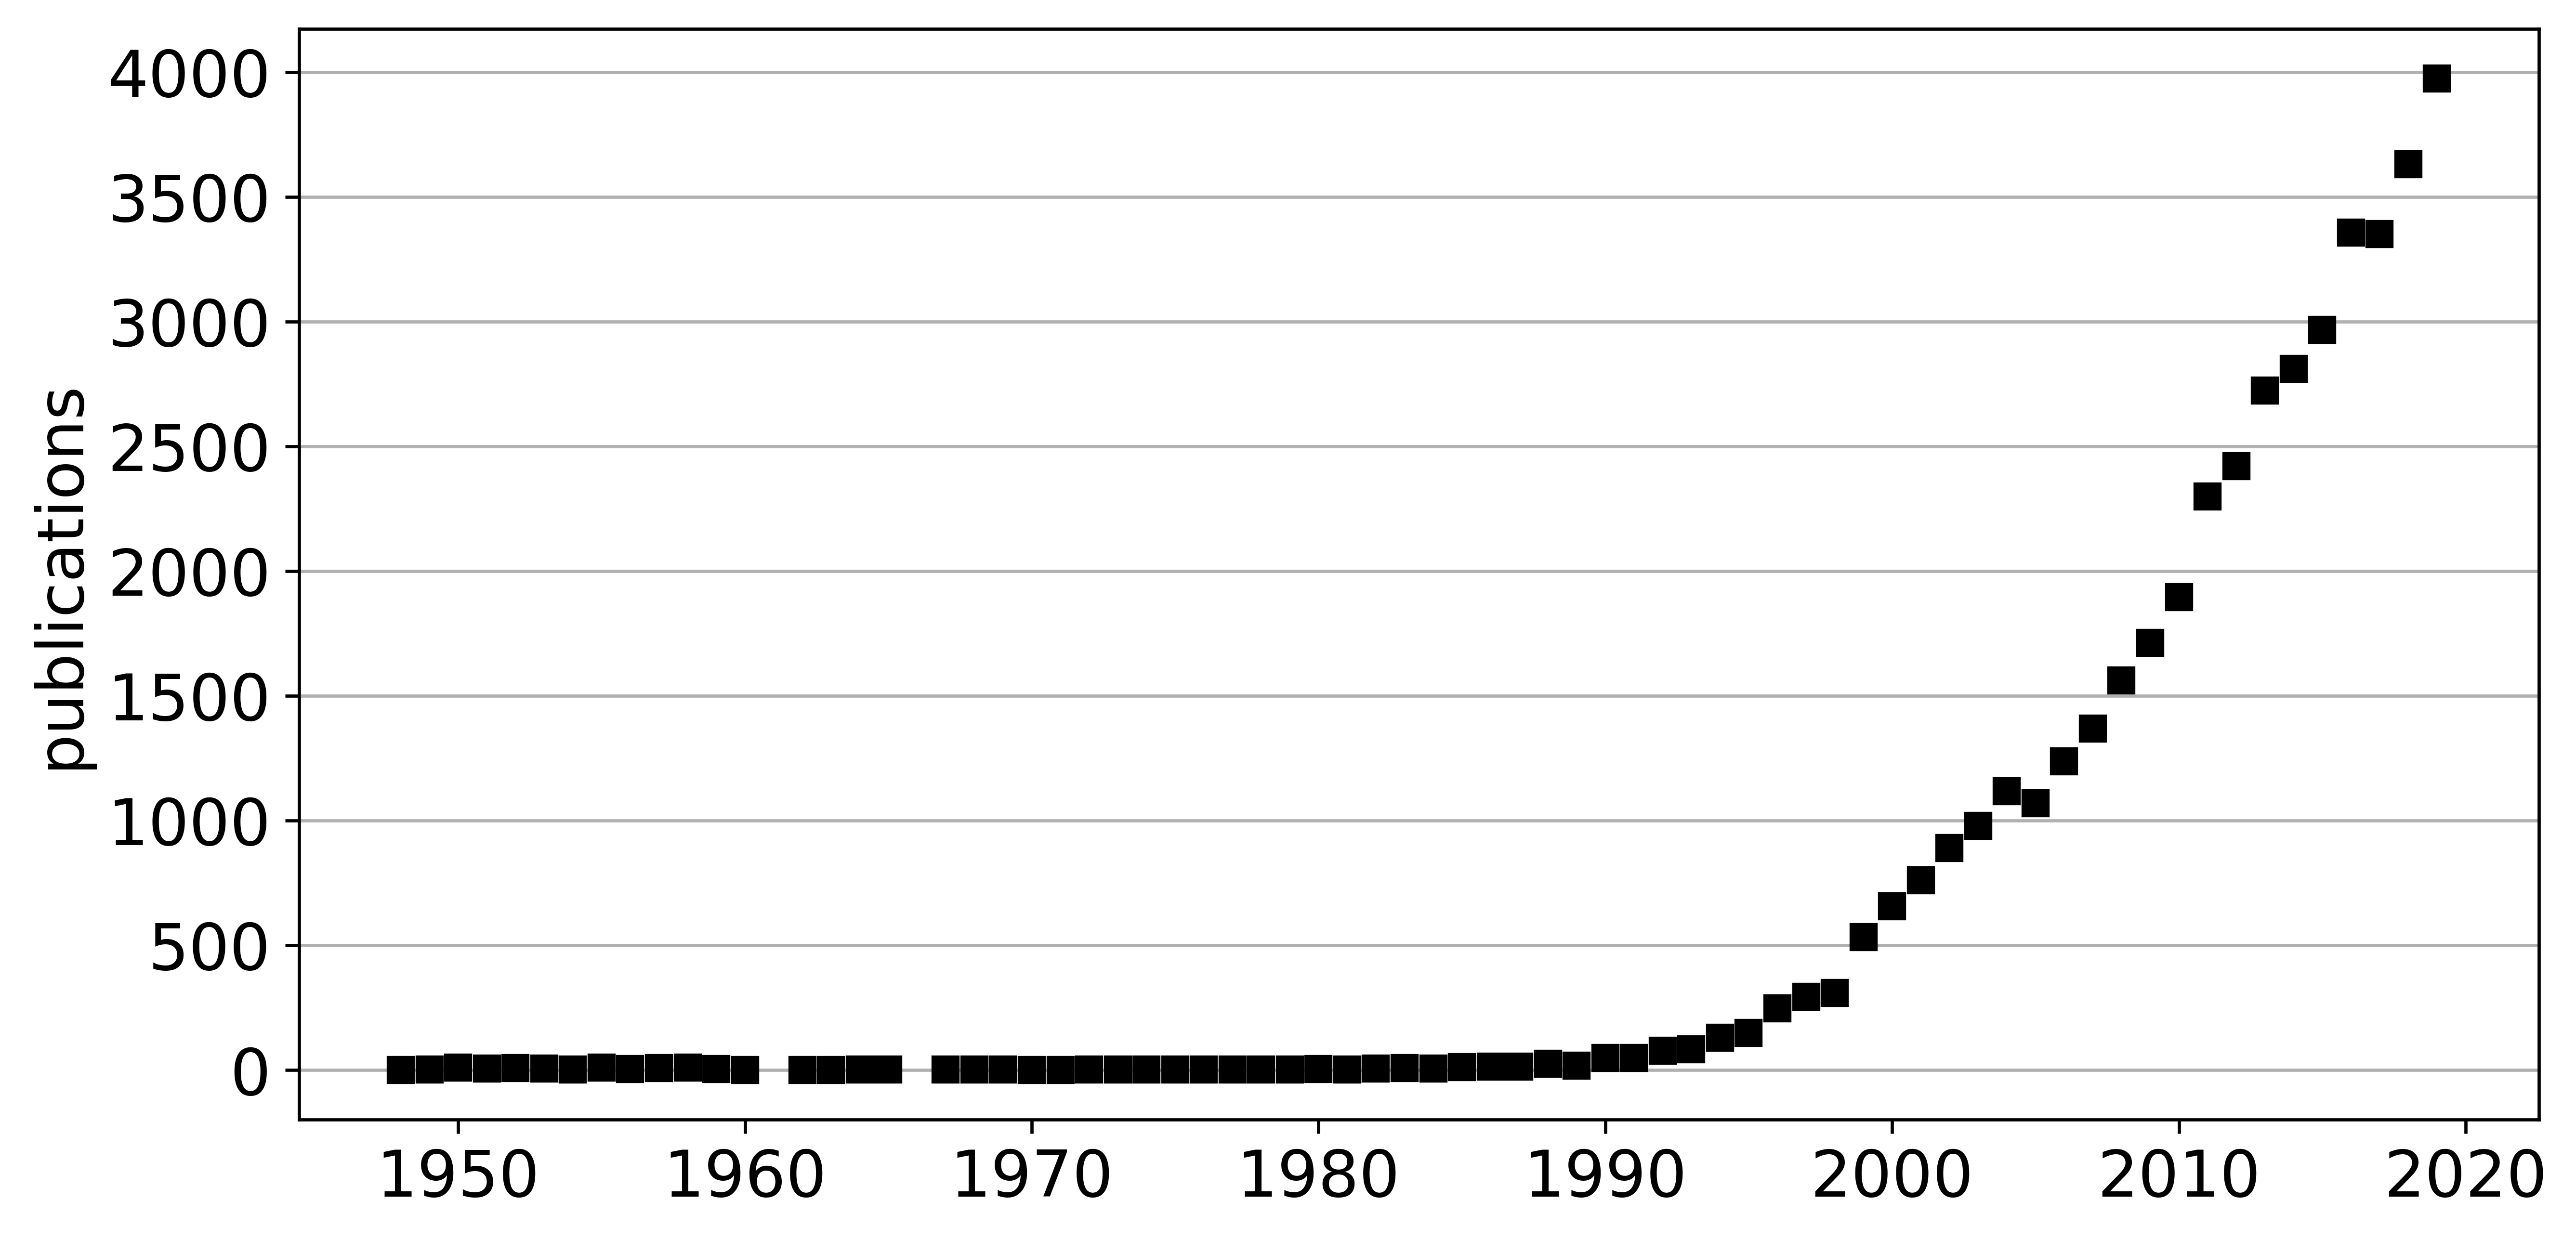
\includegraphics[width=\textwidth]{\Figures/Modeles/publis_zebra.png}
       \caption{
            \label{fig:model:pz:stats}Référencement du terme "zebrafish" au sein de PubMed
            }
\end{figure}
%
Son utilisation en tant qu'organisme modèle est fréquente pour plusieurs raisons.

    \subsection{Un modèle compact et fertile}
    
%% Petite taille
%
Le \pz{} adulte mesure environ quatre centimètres.
%
Cette petite taille présente plusieurs avantages.

%
Tout d'abord, il est possible d'élever un grand nombre de poissons dans un espace réduit~\cite{avdesh_2012}.
%%
%
Un second avantage de cette petite taille est qu'elle permet de faciliter le transport et les expérimentations avec ce modèle.
%
Il est en effet possible de transporter facilement un grand nombre d'oeufs mais aussi des juvéniles ou des adultes.
%
Cette aspect facilite le partage de lignées mutantes ou transgéniques.
%%
%
La petite taille permet aussi de manipuler facilement un grand nombre d'échantillons en parallèle~\cite{wittbrodt_2014,brion_2012}. Les pipetages à large échelle sont possibles à des stades précoces,
ce qui rend possible l'automatisation de différents traitements~\cite{mandrell_2012,teixid_2019}.

%% Reproduction
Le \pz{} possède une fertilité adaptée aux expériences impliquant un grand nombre d'échantillons.
%
Tout d'abord, la femelle pond les oeufs qui coulent au fond de l'aquarium ce  qui permet de facilement les récupérer aisément. Chaque ponte contient entre 100 et 500 oeufs ce qui permet par exemple facilement d'identifier des combinaisons de mutations dans la descendance d'un animal édité. TPS s'est doté de structures d'élevage qui permettent de caractériser près de 200 poissons en parallèle isolés dans une cage unique dans de bonnes conditions de bien-être (Marie-Elise Schwartz, TPS-AQUA, communication personnelle).  
%
Enfin, dans des conditions optimales d'élevage, le \pz{} devient fertile en environ 3 mois. Cet intervalle entre générations peut être raccourci à 2 mois pour les mâles en utilisant des robots nourrisseurs qui effectuent quatre nourrissages quotidiens, week-end y compris. 

%% Statut légal des eleuthéroembryons (EE) avant 5 jours
Le statut légal du \pz{} aux stades précoces renforce l'intérêt de son utilisation en laboratoire.
%
En effet, une espèce aquatique élevée en laboratoire rentre dans le cadre de la directive européenne n°2010/63/UE seulement à partir des stades larvaires autotrophes environ à 6dpf.
%
Cette définition permet donc de ne pas considérer les stades de développement du \pz{} entre la ponte et 5dpf comme animal de laboratoire nécessitant une autorisation d'expérimenter.
%
De plus, à ces stades, les larves de poissons-zèbre vivantes présentent une forte transparence,
ce qui permet d'imager des structures non périphériques sans réaliser de coupes~\cite{asokan_2020,chen_2020,hamilton_2016,kioka_2020}.
%%
%
Malgré tous les avantages présentés ici, l'utilisation du \pz{} en laboratoire serait limité s'il ne possédait pas un grand nombre de ressources dédiées.
%
Nous allons donc maintenant présenter certaines de ces ressources.

    \subsection{De nombreux protocoles expérimentaux sont disponibles chez le \pz{}}
    
%%
%
L'utilisation du \pz{} comme organisme modèle a pris son essor durant les années 1970~\cite{laale_1977}.
%
En 50 ans, ce modèle a ainsi été largement étudié en laboratoire.
%
En particulier, des études ont rapidement essayé de déterminer les conditions optimales nécessaires à une bonne croissance et une reproduction efficace du \pz{} en captivité, dans des conditions de bien-être acceptables~\cite{eaton_1974,eaton_1974a}.
%
De plus, la présence de longue date de cette espèce au sein des laboratoires a permis la mise en place d'au moins 34 fonds génétiques de référence pour les individus sauvages,
permettant d'étudier la diversité des génomes des individus étudiés.
%%
%
Afin d'utiliser au mieux ce modèle, de nombreux outils ont été développés.
%
En particulier, la plupart des techniques permettant de modification de génome ont été adaptées au \pz{}~\cite{auer_2014,irion_2014,foley_2009,bill_2009}.
%
Il est ainsi possible de créer facilement différents types de lignée de \pz{} génétiquement modifiées, que ce soit pour la création de lignées rapportrices~\cite{brion_2012,goldman_2001} ou pour la création de lignées KO ou KI~\cite{liu_2019}.
%%
%
Plusieurs centres de ressources et bases de données ont été créés.
%
Par exemple, le Zebrafish Internation Resource center (ZIRC), situé à Eugen en Oregon, met à disposition de la communauté plus de 43000 lignées.
%
Ce centre de référence permet ainsi d'assurer une meilleure reproductibilité des études
en permettant d'accéder à des poissons ayant un fond génétique déterminé et des insertions ou mutations validées.
%
En plus de ce centre de référence, le Zebrafish Information Network (ZFIN) est une base de données centrée sur le \pz{}.
%
Cette base de données concentre en un unique site l'ensemble des informations utiles pour effectuer des expérimentations sur le \pz{}.
%
Dans ce cadre, un catalogue de protocoles a été mis à disposition pour permettre de faciliter la diffusion des méthodes permettant de travailler avec le \pz{}.

%% Utilisation comme sentinelles environnementales ou dans le cadre de la tératologie
%
Ce modèle est aussi référencé par des institutions gouvernementales pour le développement d'essais toxicologiques.
%
L'OCDE a ainsi émis différents protocoles visant à standardiser son utilisation pour l'étude de la toxicité aiguë pour les embryons~\cite{oecd_2013}. Ces tests peuvent mesurer la toxicité à de courtes expositions durant les stades précoces (embryon et eleutheroembryon)~\cite{oecd_2013a} ou bien étudier  des stades plus tardifs, et par exemple caractériser les défauts de croissance juvénile suivant l'exposition à des molécules toxiques~\cite{oecd_2000}.
%
La directive REACH de l'Union Européenne, qui vise à réglementer les études des risques liés aux substances chimiques, se concentre particulièrement sur l'étude des perturbateurs endocriniens.
%
Dans ce cadre, une méthode de mise en évidence de l'activité endocrine d'une substance chimique sur des EEs de \pz{} est reconnue comme méthode de référence\cite{europeanchemicalagencyechaandeuropeanfoodsafetyauthorityefsawiththetechnicalsupportofthejointresearchcentrejrc_2018}.

Il ne fait pas de doute que le  pertinence du \pz{} pour détecter d'éventuels effets délétères de molécules chimiques sur les poissons des rivières et même les poissons marins. En revanche, du fait de la distance évolutive avec l'homme, les conclusions tirées d'études sur le \pz{} ne peuvent constituer que de premiers éléments  qui doivent être confirmés par des tests sur d'autres espèces , bien évidemment des mammifères, mais aussi des amphibiens. En cas de caractérisation d'effets toxiques d'une molécule sur les stades précoces, on peut considérer le \pz{} comme un lanceur d'alerte concernant le potentiel tértogénique de cette molécule en particulier. En aucun cas, l'absence d'efffet ne peut être une preuve de son inocuité. 
    
    \subsection{De nombreuses applications en recherche biomédicale}

%
Le \pz{} possède 80\% de gènes homologues communs avec l'humain~\cite{howe_2013}. 
Ce taux d'homologie permet d'utiliser le \pz{} pour la modélisation d'un certain nombre de maladies humaines.
En particulier avec l'apparition des dernières méthodes d'édition du génome permettant d'introduire des mutations ponctuelles par réverse transcription ("base editing", ref), il est possible de modéliser les maladies humaines avec précision chez le \pz{}, en introduisant chez le \pz{} des variations à des positions orthologues chez l'humain où se trouvent des variations génomiques pathogènes.
Bien entendu, ces modèles, en particulier du fait de leur capacité à effectuer de la microscopie à haut-contenu et haut-débit contribuent à la compréhension des mécanismes physio-pathologiques, du génotype au phénotype, et à éclairer comment une mutation entraîne des effets cellulaires ciblés et parfois discrets sur le long terme , dans le cadre de l'organisme entier.
Ils permettent aussi permettre d'effectuer des études pré-cliniques visant à déterminer des cibles thérapeutiques, voir tester des traitements contre ces maladies~\cite{vaz_2018,pitchai_2019,saleem_2018} en particulier les thérapies innovantes utilisant des cellules souches ou immunitaires, ou des méthodes d'édition du génome. 
%
Une grande diversité de maladies sont abordées, car l'EE et les juvéniles possèdent des organes très similaires à l'humain, même s'ils sont de plus petite taille et considérablement simplifiés. On peut par exemple citer les maladies neurodégénératives~\cite{fontana_2018}, les anomalies du développement~\cite{lovely_2016,sarmah_2016} ou les maladies cardiaques~\cite{brown_2016, walcott_2014}.

\section{Autres modèles animaux\label{sec:intro:modele} pouvant tirer profit des résultats de ma thèse}

Nous allons maintenant présenter trois espèces par ordre croissant de divergence avec le \pz{}: \ol, \xl{} et \mm{}.

    \subsection{\label{sec:medaka}le médaka, un modèle complémentaire au \pz{} très utilisé en toxicologie}
    
%
Le médaka est un poisson téléostéen originaire d'Asie du Sud-Est.
%
Il est de taille comparable au \pz{} et présente une gestation courte et prolifique.
%
Sa capacité à résister au froid, et son développement embryonnaire, non pas de 48h comme chez le \pz{} mais de l'ordre de dix jours,  facilite son transport, permettant ainsi par exemple pour une plateforme de facilement distribuer des oeufs à d'autres laboratoires.
%
Plusieurs outils de modification du génome ont été mis en place chez \ol{}\cite{kirchmaier_2015, ansai_2017}, 
ce qui permet la création de lignées rapportrices, de lignées knock-out et de lignées knock-in\cite{abdelmoneim_2018,jin_2020,Watakabe_2018,qiu_2014,gay_2018}.
%
Enfin, à l'instar du \pz{} avant 120 heures post fertilisation,
le médaka avant 240 heures post-fécondation n'est pas autotrophe.
%
Les embryons et eleutheroembryons ne sont donc pas dans le périmètre de la directive 2010/63/EU de l'Union Européenne.
%
Ainsi, ces stades ne font pas l'objet de demande d'expérimentation animale avant tout projet étant susceptible d 'induire une douleur.

%
C'est aussi un poisson très résistant, qui possède un génome plus compact que le \pz{} , est très distant évolutivement de ce dernier (plus de distance qu'entre le poulet et l'homme), de très bons taux en édition du génome du fait de la possibilité de refroidir l'oeuf. Il possède aussi de nombreuses sous espèces ou espèces soeurs , dont certaines sont maarines, ce qui permet de très intéressantes études comparées.
%
On retrouve ainsi les premières publications utilisant \ol{} dès 1921\cite{aida_1921}.
%
Son utilisation dans le cadre de publications scientifiques reste assez faible, avec en moyenne deux cents publications annuelles référencées par PubMed(voir Figure~\ref{fig:model:oz:stats}).
%
Mais il est par exemple utilisé dans l'étude du système reproducteur~\cite{gay_2018,herberg_2018} ou
en toxicologie~\cite{carvan_2007,bertotto_2019,cleary_2019,powe_2018}.
%
En particulier, son utilisation dans l'étude des perturbateurs endocriniens a été l'objet d'un protocole de l'OCDE~\cite{oecd_2009}, en faisant un organisme de choix dans l'étude de l'activité endocrine d'une molécule~\cite{chen_2018,dang_2019,spirhanzlova_2016}.

\begin{figure}[htbp]{\textwidth} 
    \centering
       \centering 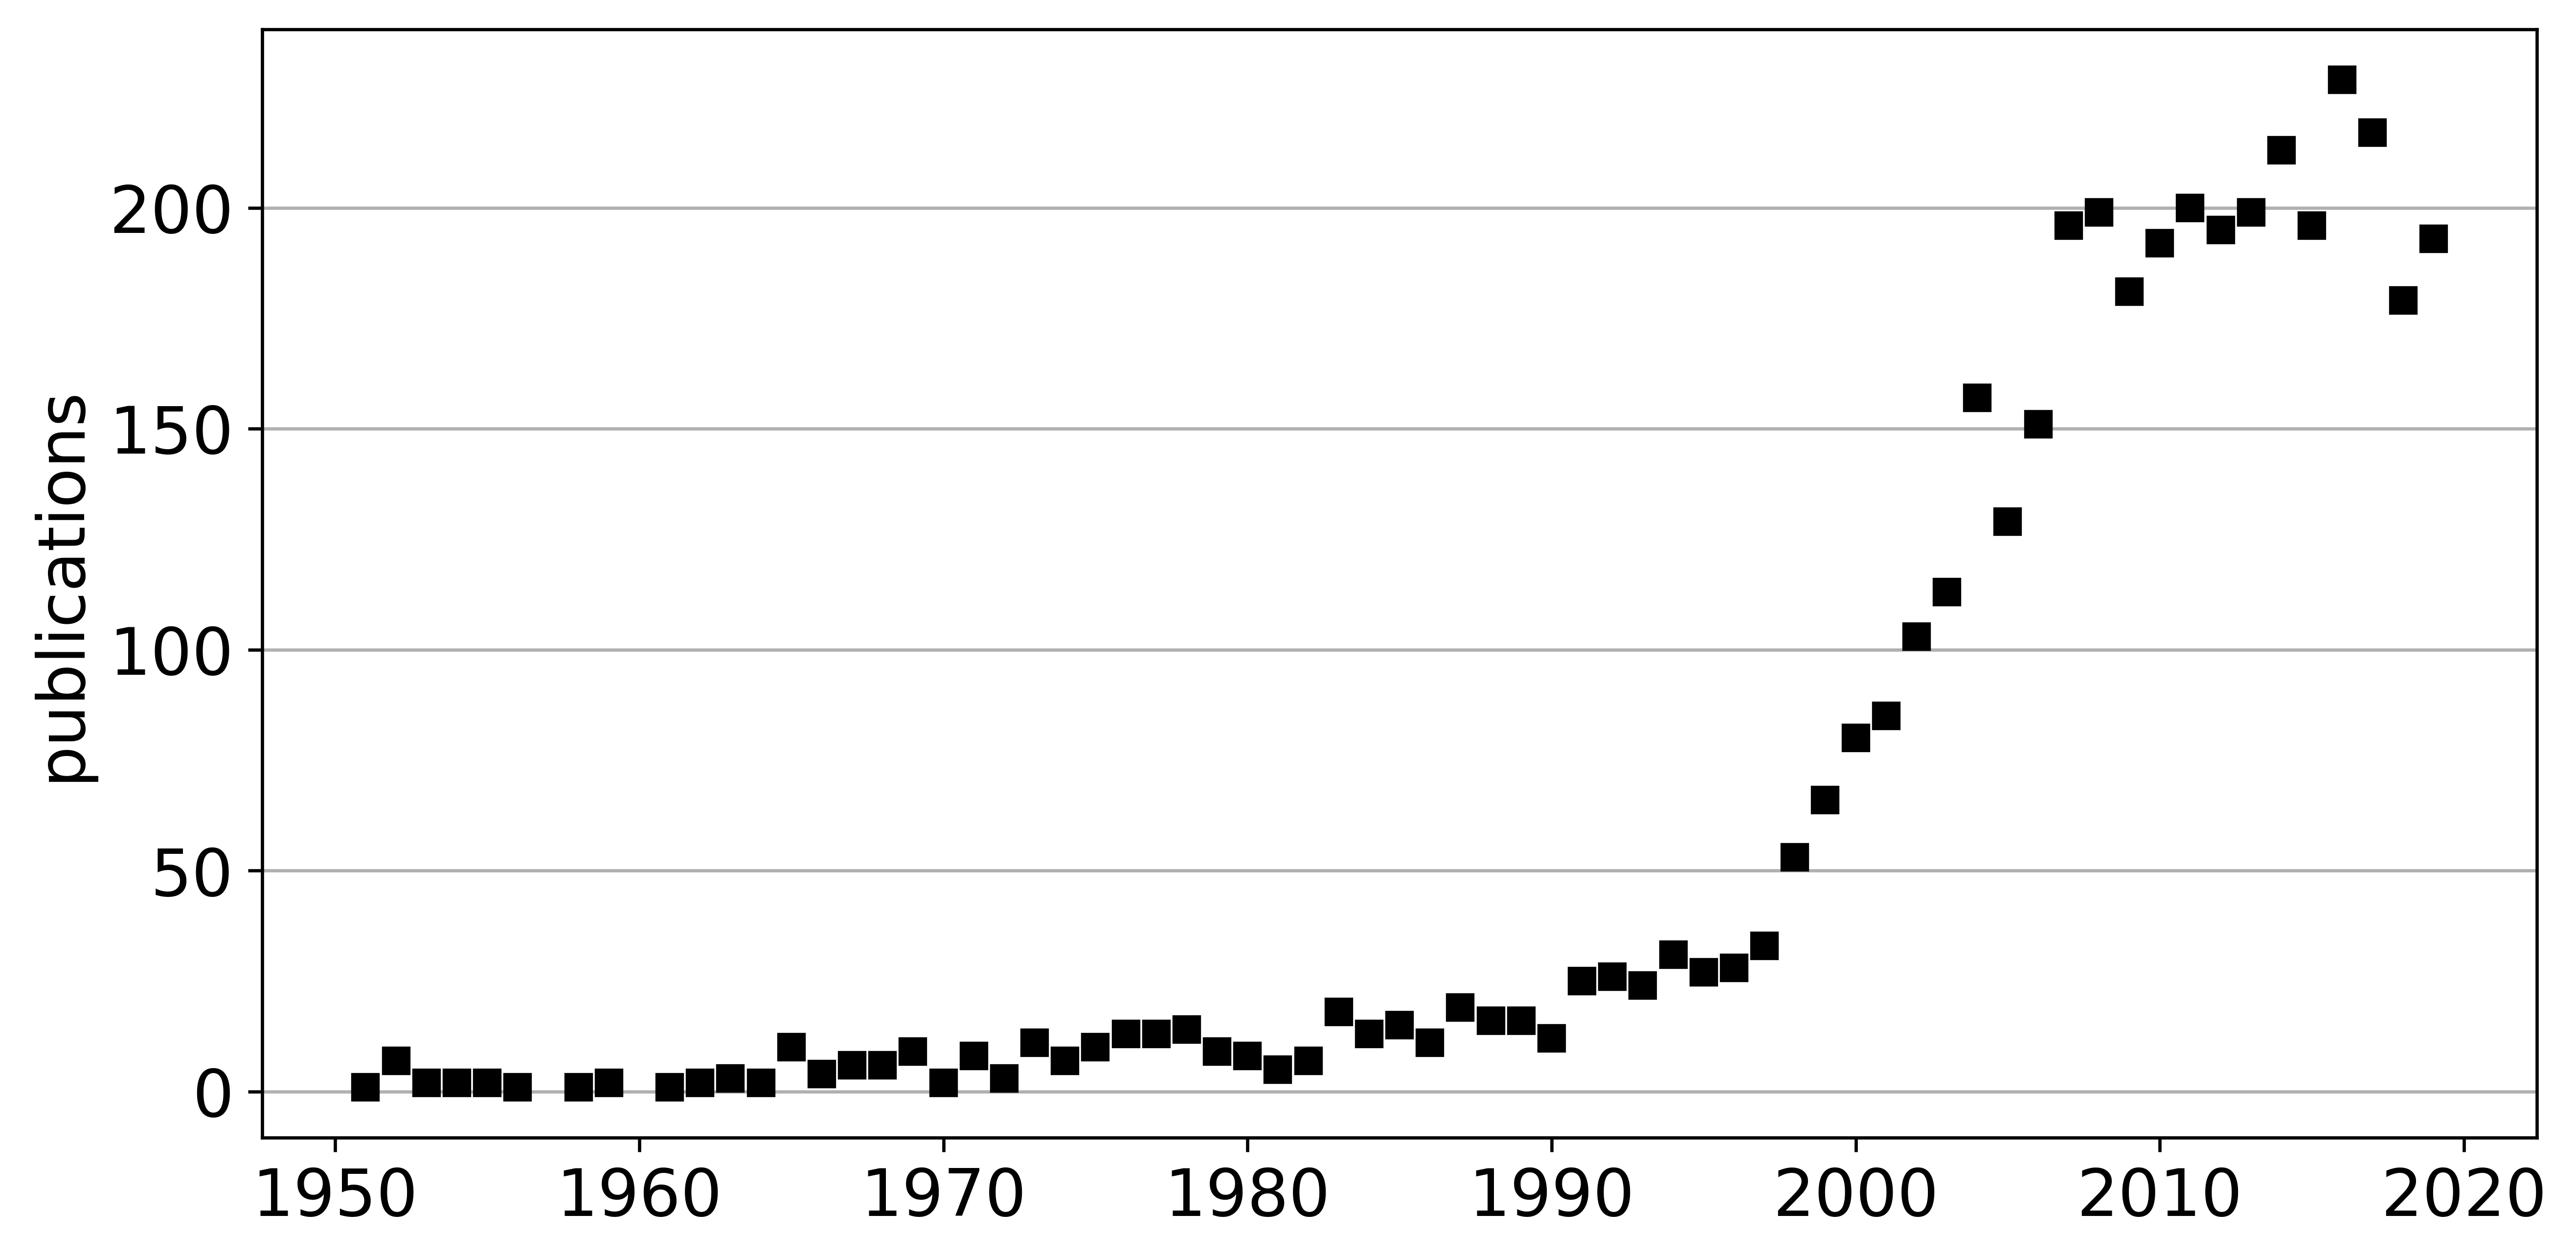
\includegraphics[width=\textwidth]{\Figures/Modeles/publis_medaka.png}
       \caption{
            \label{fig:model:oz:stats}Référencement du terme "medaka" au sein de PubMed
            }
\end{figure}

Les premières utilisations du médaka dans le cadre de \hcs{} sont référencées dès les années 1980~\cite{cameron_1985,Hatanaka_1982}.
%
Cependant, il s'agit d'un organisme rarement référencé pour le \hcs{} par imagerie~\cite{gierten_2020,genest_2019}.

%
Il est pourtant possible d'utiliser un système d'imagerie développé sur le \pz{}
en effectuant peu de modifications pour le faire fonctionner sur le médaka.

    \subsection{le xénope, un modèle de référence en biologie du développement}

%
\xl{} est une espèce d'amphibiens originaire respectivement d'Afrique de l'ouest et d'Afrique australe.
%
Bien qu'une femelle ne puisse être stimulée pour la reproduction que tous les trois mois,
sa capacité à produire jusqu'à 4000 oeufs par ponte permet d'avoir rapidement un grand nombre d'échantillons.
%
Elle est en particulier connue du grand public pour être la base d'un des premiers procédés de détection de grossesse chez l'humain dans les années 1950~\cite{hobson_1958,Dittebrandt_1949,polack_1949}
et pour avoir servi de modèle pour le clonage , ce qui a été récemment récompensé en incluant aux côtés d'autres chercheurs \textsc{John Gurdon}  dans un prix Nobel attribué au clonage.
%
Il s'agit d'un organisme modèle donc établi de très longue date dans la communauté scientifique.
%
Les premières publications scientifiques l'utilisant date de 1930~\cite{edgeworth_1930},
et plus de 1000 publications y faisaient dès l'an 2000.
%
Son utilisation est cependant en baisse au vue de la baisse de référence à partir de 2010. (voir Figure~\ref{fig:model:xl:stats}).
%

\begin{figure}[htbp]{\textwidth} 
    \centering
       \centering 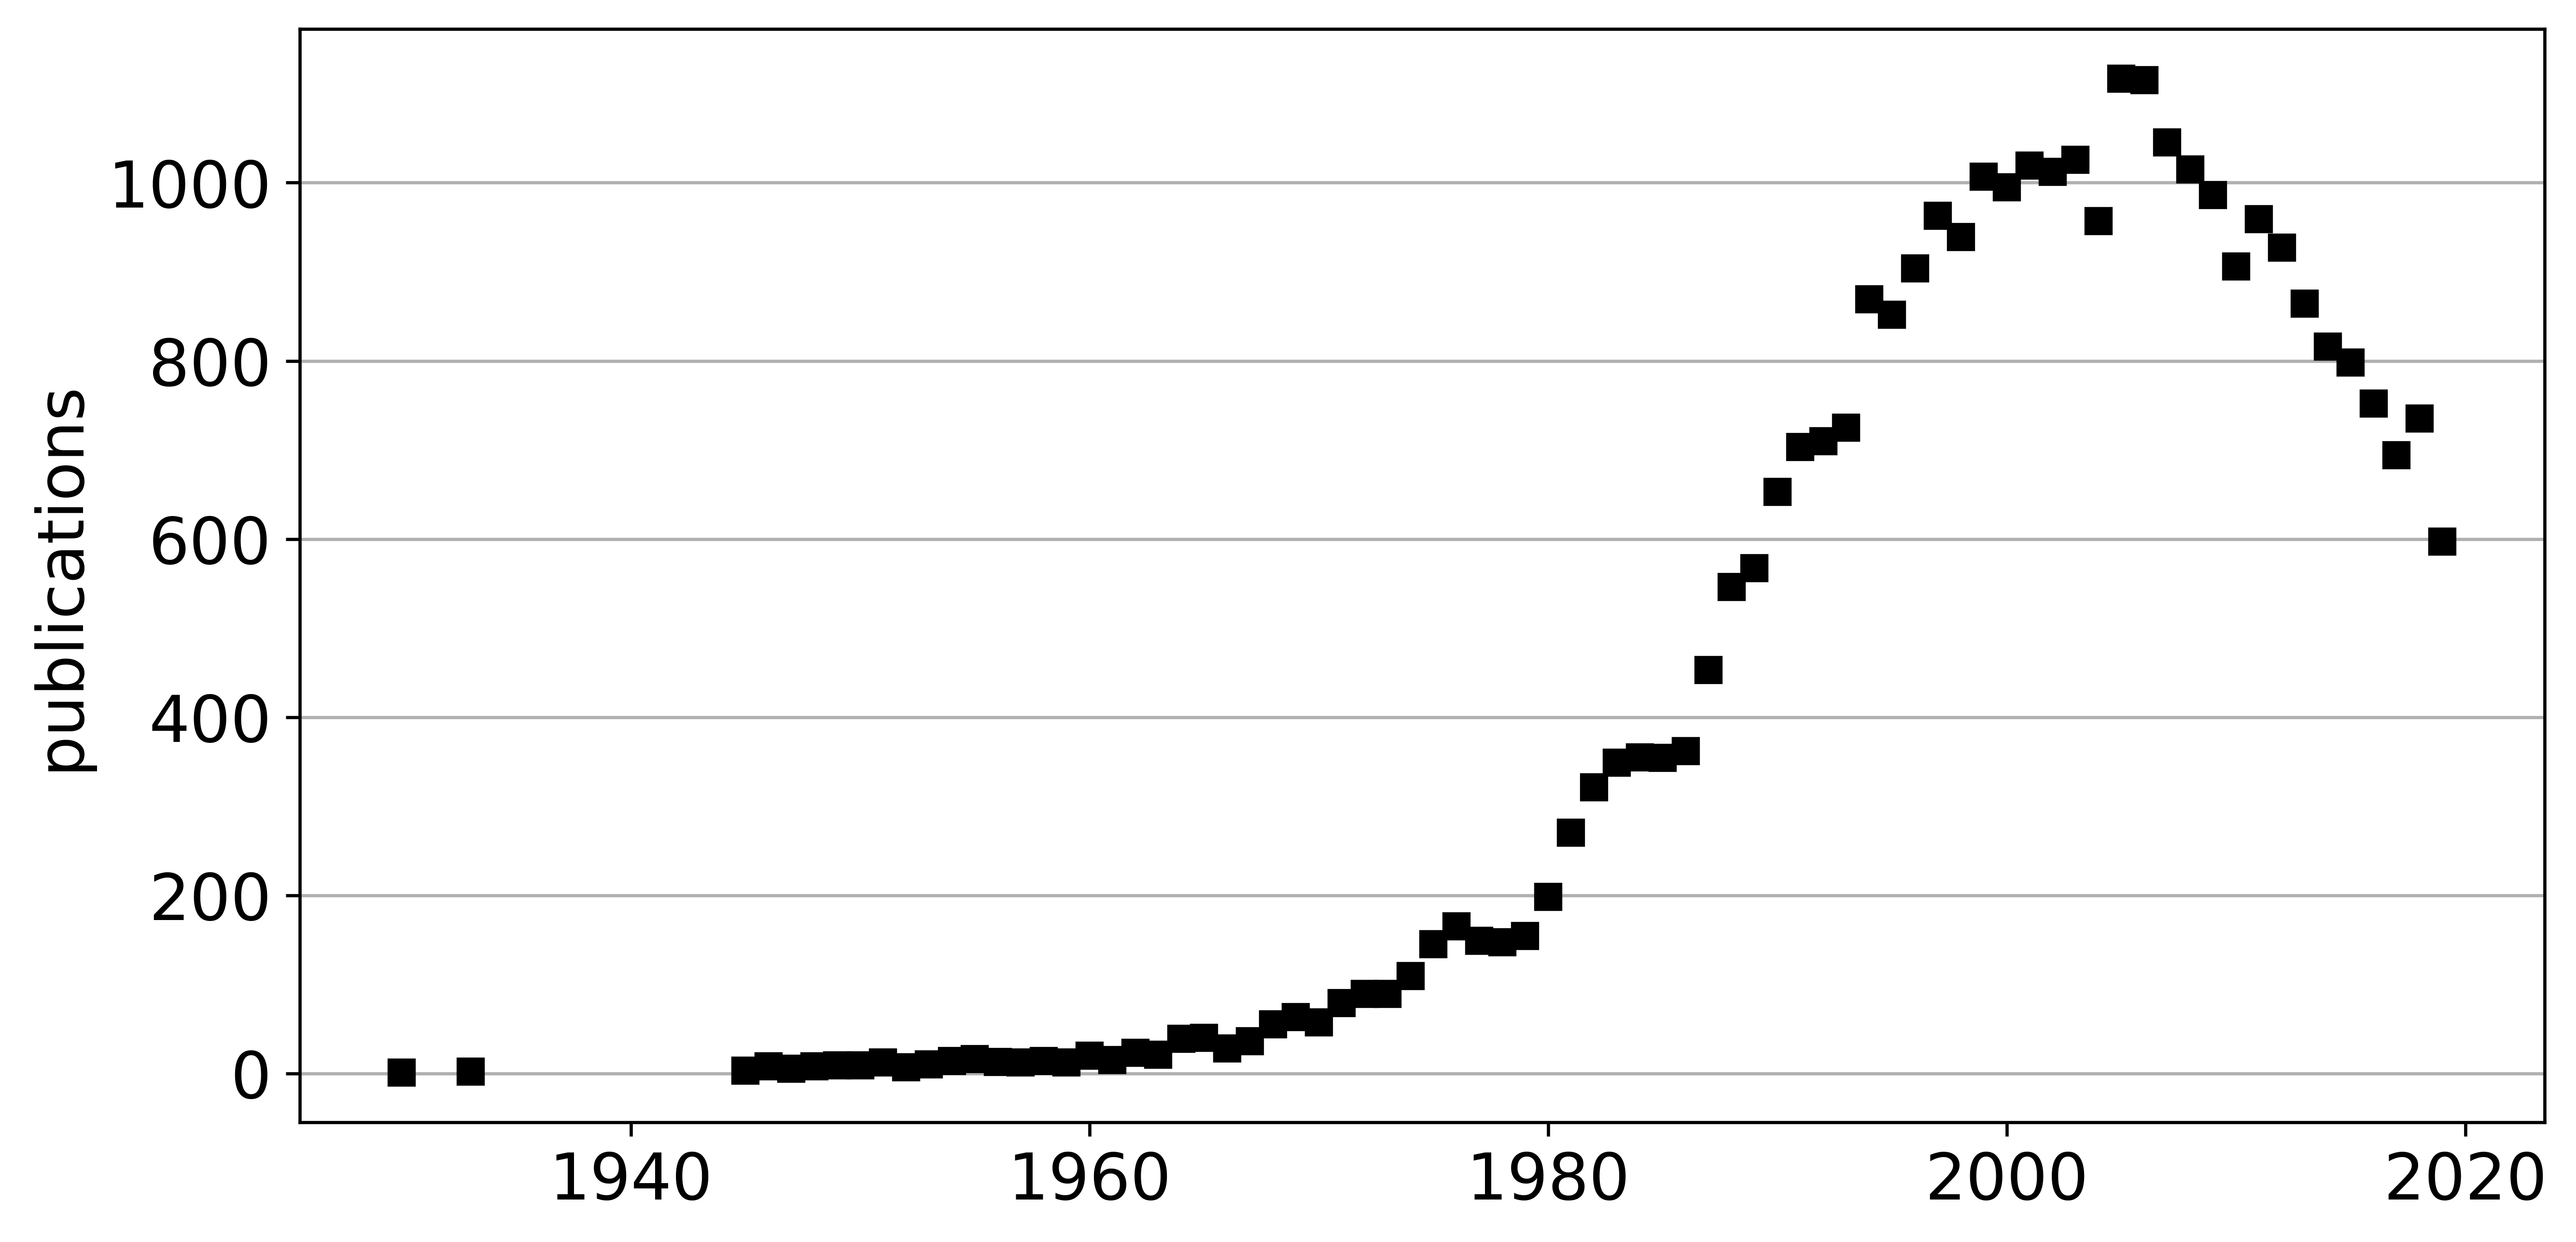
\includegraphics[width=\textwidth]{\Figures/Modeles/publis_xenopus.png}
       \caption{
            \label{fig:model:xl:stats}Référencement des termes "xenopus laevis" au sein de PubMed
            }
\end{figure}

%%
%
\xl{} est un modèle d'intérêt pour plusieurs domaines.
%
Il s'agit par exemple d'un modèle de référence dans l'étude du système visuel~\cite{viet_2020,Rahman_2020,kha_2020},
en particulier grâce à sa capacité de régénération de la lentille de l'oeil après ablation de cette lentille~\cite{henry_2019}.
%
Le passage de l'état de têtard à l'état juvénile, appelé métamorphose, est contrôlé chez \xl{} par des hormones thyroïdiennes~\cite{brown_1996,furlow_2006}.
%
Cette particularité rend ce modèle particulièrement intéressant dans l'étude des perturbateurs thyroïdiens~\cite{li_2019,li_2019a,Couderq_2020}.
%
Enfin, \xl{} ne développe que peu de cancers spontanés~\cite{ruben_2007} mais il est possible d'induire la formation de tumeurs. Ces caractéristiques en font un modèle de choix aussi bien dans l'étude de la réponse immunitaire anti-tumorale que dans le développement des cancers~\cite{hardwick_2015}.
%
 Ces dernières années, le développement de méthodes de transgénèse chez \xl{}~\cite{tandon_2017} a permis la mise en place rapide de lignées rapportrices ou de lignées permettant l'étude de mutations responsables de maladies humaines.

    \subsection{La souris, un modèle omniprésent en neuroscience}

La souris est l'organisme vertébré le plus étudié en laboratoire.
%
Son utilisation  est décrite dès le dix-septième siècle.
%
Plus de 80000 publications référençaient ce modèle en 2019 (voir Figure~\ref{fig:model:mm:stats}).

\begin{figure}[htbp]{\textwidth} 
    \centering
       \centering 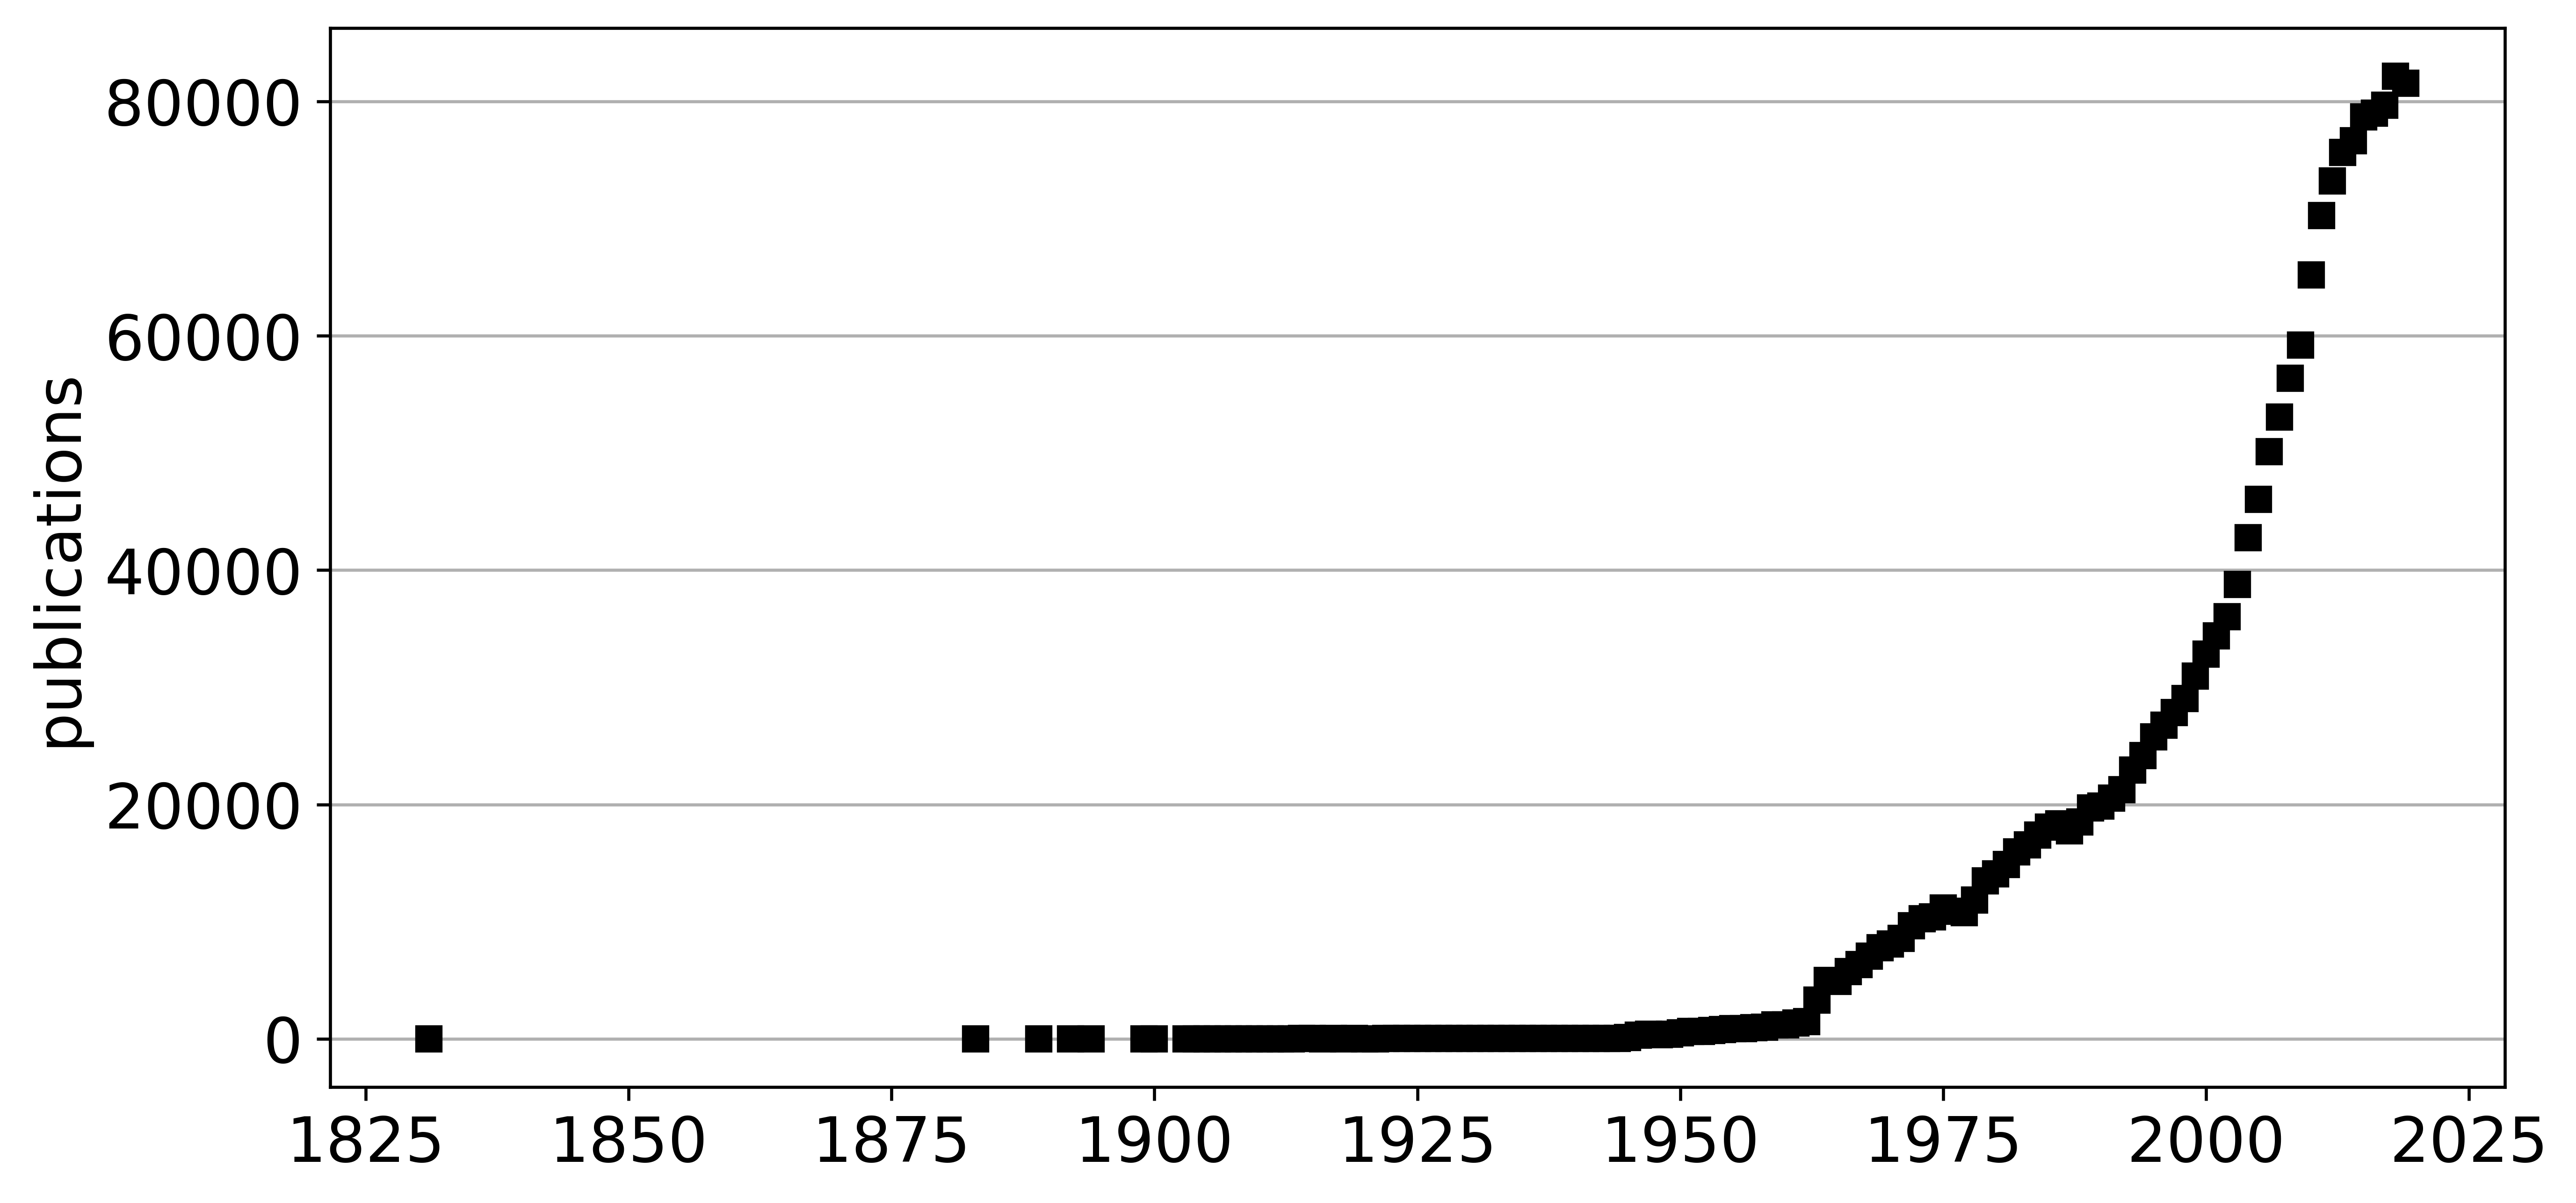
\includegraphics[width=\textwidth]{\Figures/Modeles/publis_mus.png}
       \caption{
            \label{fig:model:mm:stats}Référencement des termes "mus musculus" au sein de PubMed
            }
\end{figure}

%
Les outils permettant la modification de son génome sont largement développés~\cite{lanigan_2020}.
%
Il est donc possible de modifier le génome de souris pour pouvoir utiliser ce modèle comme outil d'étude de pathologie humaine.
%
Par exemple, la souris est régulièrement utilisée pour étudier diverses maladies neurodégénératives,
comme la maladie d'Alzheimer~\cite{han_2020,thadathil_2020,shin_2020},
la sclérose latérale amyotropique~\cite{Ahmed_2020,konopka_2020,mcleod_2020}
ou la maladie de Huntington~\cite{deng_2020,dridi_2020,pfister_2020}.

\end{document}